\documentclass{stdlocal}
\begin{document}
\section{Tests, Benchmarks and the Simulation of Photons} % (fold)
\label{sec:testing_framework}

  \subsection{Functionality and Correctness} % (fold)
  \label{sub:unit_tests}
    While working on modules of a library, we always have to make sure to test their functionality.
    Typically, this is done via unit and integration tests.
    We do not want to go into details of testing but instead want to show a few unit tests that were created and used during the development process.
    Besides consistency and correctness, this will additionally show how to apply the library in other code.
    To append and create new tests easily, a unit testing framework called \citetitle{doctest} was used \autocite{doctest}.
    Because all PRNGs are in general tested the same way, we will only describe the testing facilities by means of the MT19937 and AVX intrinsics if not otherwise stated.

    \inputCodeBlock[title = Scalar MT19937 Advance Test]{code/mt19937/sisd/test.cpp}
    In our scalar implementation of the MT19937, we wanted to guarantee that its output does not differ in comparison to the output of the \code{std::mt19937} of the STL of C++.
    Using only the seeding process and the advancing methods of the generators, we came up with the most simplest solution.
    We use a truly random seed given from \code{std::random\_device} to initialize the standard Mersenne twister from the STL and our own implementation the same way.
    Afterwards, we are requiring the equality of their output for several million calls to the function operator.
    It does not necessarily fulfill all good design principles for unit tests but asks for enough information, such that multiple successful runs of this test imply the correctness of the implementation.
    Therefore, we avoided an infeasible brute-force method of testing all possible outputs.
    As we have designed another API, our own Mersenne twister has to be seeded with its default seeder, such that it is able to use only one 32-bit random number in the construction process.
    Please note, \code{std::random\_device} does not have to be truly random \autocite{oneill-blog-rd,oneill-blog-seeding-surprises} but could be replaced by other seeding alternatives if this should be the case \autocite{oneill-blog-seed-entropy}.

    Testing the vectorized implementation of an advancing method can be done the same way by comparing each element of an SIMD vector with the output of the scalar version.
    The code for this is given the appendix in listing \ref{code:mt19937-avx-advance-test}.
    The use of appropriate \code{using} declarations makes the code more readable.
    As a special case, the vectorization of the jump function of the Xoroshiro128+, given in listing \ref{code:xoroshiro-avx-jump-test}, can be tested by checking the equality of the internal state variables after successfully testing its advancing routine.
    Here, we have to take care when initializing the four scalar instances to test against.
    We first set their state directly to be able to run the comparison the same way after doing the jump.

  % subsection unit_tests (end)

  \subsection{Randomness of Multiple Streams} % (fold)
  \label{sub:statistical_testing}
    The topic of this thesis is not to develop new PRNGs.
    As a consequence, we will not test the statistical performance of the already known scalar PRNGs.
    Instead, we have to examine the randomness of the created multiple streams embodied by the SIMD vectors.
    As stated in \textcite[\ppno~160-162]{kneusel2018}, we will combine all streams of random numbers into a single one by interleaving the samples as shown in figure \ref{fig:combined-stream}.
    The combined stream will then be used as an input to the common test suites \citetitle{testu01-lib} and \citetitle{dieharder} \autocite{testu01,dieharder}.
    \begin{figure}
      \center
      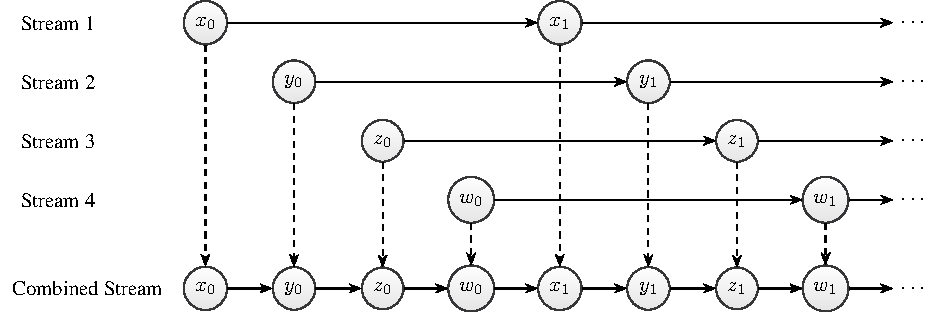
\includegraphics[width=0.95\textwidth]{figures/interleaving_multiple_streams.pdf}
      \caption[Combined Stream by Interleaving Samples of Multiple Streams]{%
        Interleaving samples of multiple streams of random numbers to produce a combined stream which can be used as input for common statistical test suites.
        Modeled after \textcite[\pno~161]{kneusel2018}.
      }
      \label{fig:combined-stream}
    \end{figure}

    By using the described method, testing vectorized PRNGs which use the leapfrogging method to generate multiple streams will not give us further insights to their randomness properties because interleaving the samples would produce the same output as the scalar version.
    Especially, this is true for the MT19937.
    Hence, we only test the output of the vectorized Xoroshiro128+ and the MSWS to guarantee the vectorization process is not reducing the statistical performance of the generators.
    We will not test the jump initialization of the Xoroshiro128+ as it was already tested by \textcite{vigna-xoroshiro}.
    The process of testing was geared to \textcite[\ppno~141-155]{kneusel2018} and \textcite{oneill-blog-testu01}.

    \subsubsection*{Test Suite \citetitle{dieharder}}
    To test external RNGs with the \citetitle{dieharder} test suite, the typical approach is to generate a stream of random bits which will be used as input for the test suite by using a pipeline on the command line.
    The following code snippet provides a bit stream for the AVX implementation of the Xoroshiro128+ by writing its binary output to the standard output.
    The given implementation can be easily adjusted to work with the other generators by changing the type of the PRNG.

    \inputCodeBlock[title = AVX Xoroshiro128+ Bit Stream]{code/xoroshiro128plus/simd256/bitstream.cpp}
    The \code{main} procedure starts with two statements that speed up the output process by first disabling the synchronization between the C and C++ IO streams and then untying the standard output stream \code{cout} from the standard input stream \code{cin}.
    We do not want to mix C and C++ IO operations and we do not need a thread-safe output stream so that disabling syncing should make the code faster \autocite{cppreference}.
    Because our bit stream will only use the output operation independently from any input routine we make sure the usage of \code{cin} will not flush the buffer of \code{cout} to further raise the speed of the output \autocite{cppreference}.
    Afterwards, we initialize the generator by the TRNG \code{std::random_device} of the C++ STL and use an infinite loop to write its output to \code{cout} in binary form.
    For this, we first generate a new random number by advancing the state of \code{rng} and the calling \code{cout.write}.
    Using the compiled program as input for the \citetitle{dieharder} test suite can be done on the command line in the following way.
    \[
      \text{\code{bench/xrsr128p_simd256_bitstream | dieharder -a -g 200}}
    \]

    \subsubsection*{Test Suite \citetitle{testu01-lib}}
    \citetitle{testu01-lib} is a software library written in the C programming language and can be directly used inside a C++ program.
    Because we have designed a C++ API for our vectorized generators and TestU01 is only able to read a continuous sequence of 32-bit random numbers, we have to wrap their output in a C-compatible way by using functions and global variables.
    The following code snippet shows again the easiest possible implementation for the vectorized Xoroshiro128+.
    By the changing the type of the RNG, other generators can be tested as well.
    Please note, there are much more advanced methods to use TestU01 in C++ code but we only wanted to show the essential parts.

    \inputCodeBlock[title = AVX Xoroshiro128+ TestU01]{code/xoroshiro128plus/simd256/testu01.cpp}
    To make sure that we supply a sequence of 32-bit values without changing the actual output of the RNG, a wrapper function is used to serialize larger random values.
    We are using a small cache which stores the last generated random value.
    By calling \code{serializer}, we go to the next 32-bit chunk of data inside the cache and return those values.
    When we reach the end of the cache, we advance the actual generator and again store its value inside the cache and start anew.
    Both, generator and cache, are stored as global variables to reduce their access time in comparison to \code{static} variables inside the function \code{serializer}.

    In the \code{main} function, arguments given on the command line decide which test battery to run.
    We allocate a TestU01 generator given by an external function through the call of \code{unif01_CreateExternGenBits}.
    Afterwards, we run one of the chosen test batteries, Small Crush, Crush, or BigCrush.
    At the end, \code{unif01_DeleteExternGenBits} deallocates the external generator.

    The given procedure to serialize random output which is larger than $32\appendUnit{bit}$ is not unique and will not be able to uncover all possible statistical flaws \autocite{oneill-blog-testu01}.
    But an exhaustive variant of testing is quite time-intensive and will make the results much more complicated to interpret.
    In the end, there will always be statistical and empirical tests which will detect the deterministic behavior of PRNGs.
    As a consequence, the required statistical quality heavily depends on the application a PRNG is used for.
    For our purposes, the given testing process is completely sufficient.
  % subsection statistical_testing (end)

  \subsection{Generation Benchmark} % (fold)
  \label{sub:generation_benchmark}
    Benchmarking the generation of random numbers is tricky.
    We have encountered several inconsistencies when measuring and comparing the speed of different PRNG implementations.
    In general, small adjustments in the code of the benchmark completely changed the behavior and performance of the scalar PRNG versions.
    Furthermore, even the order of PRNGs affected the performance of several generators.
    Due to the compiler optimization process, some implementations of scalar PRNGs will be optimized with a varying effectiveness while used in different benchmarking scenarios.
    Sometimes the compiler will notice that computed values are not needed by other parts of the program.
    As a result, it will optimize the code such that the PRNG to be measured will never be called.
    Of course, this completely falsifies the performance measurement and makes comparisons impossible.
    Hence, we recommend to measure the performance of random number generation in an actual application.

    The following benchmark which is split into three smaller parts was designed to be independent of the order of PRNGs.
    Advancing the state of a generator is forced by using an underlying cache with a capacity of several thousands of bytes in which random numbers will be stored.
    The compiler is not allowed to remove the cache by means of optimization.
    With the benchmark, it is possible to measure the speed-up introduced by vectorization.
    We used the \citetitle{perfevent} benchmarking wrapper to simplify the implementation of the measurement process.
    Additionally, it gives us further insights, such as the average instructions per cycle (IPC), average branch misses, average cache misses, and even more \autocite{perfevent}.

    To apply the benchmarking routine easily to any possible generator, we use an abstraction class, given in listing \ref{code:generation-benchmark-structure} in the appendix, which saves the context variables, such as the number of samples and the \citetitle{perfevent} parameters.
    The member function templates \code{run} are used to actually execute the benchmarking routine and write the results to the standard output.
    We overload the template to automatically deduce the type of a given RNG and the algorithm to use.
    Because on modern systems the \code{std::mt19937} of the C++ STL uses a 64-bit integer type to output a 32-bit random number, we have to introduce the possibility of manually setting the type the return type will be casted to.
    To not always specify it explicitly, the second overload makes sure to automatically deduce the return type by the use of \code{decltype}.
    The third and the fourth variant implement the same benchmarking routine for two generators of the same type by alternately advancing their states and writing their output into the cache.
    We use this facility to compare the performance of a single PRNG instance to the that of two instances used at once which may give us further insights into latency- and throughput-based issues.

    \inputCodeBlock[title = Generation Benchmark Implementation]{code/generation_benchmark/benchmark.hpp}
    Above, we only show the benchmark implementation for a single instance of a PRNG.
    The version using two instances follows directly from the given code.
    At first, we add \citetitle{perfevent} parameters, like the name of the PRNG, to get a more detailed output on the command line for every measurement.
    Afterwards, the cache which is preventing the removal of the call to the PRNG by compiler optimization is initialized.
    To warm up the cache, several thousand random numbers will be generated and stored in the cache without measuring performance.
    With this, we make sure the state of the PRNG and the cache already lie inside the L1 or L2 cache of the computer hardware if possible.
    The insertion of a warm-up process greatly reduced the noise of measurements between multiple benchmark runs.
    Then we start a new scope that is used for the actual benchmark.
    We construct a \code{PerfEventBlock} that immediately starts with the measuring process.
    Due to the RAII principle of C++, the \code{PerfEventBlock} will be destroyed at the end of the scope finishing the measurements and outputting the results.
    Between its construction and destruction, we run over the cache filling it with random numbers generated by the PRNG again and yet again.
    Typically, the time for only one call to the advancing routine of a generator is unmeasurable because it is too fast.
    Hence, we accumulate the time needed for several thousand calls and calculate the average time needed for the generation of one number.

    To easily use the benchmarking structure for multiple runs with different RNGs, we always return a reference to itself.
    This allows us to chain the calls in the \code{main} function reducing the usage overhead.
    The code is given in listing \ref{code:generation-benchmark-usage}.
    Inside the \code{main} function, the sample count is read from the command line and then put into the constructor of \code{benchmark}.
    Afterwards, a list of runs for different generators exploiting the single and double instance facilities is given with the help of the chaining mechanism.
    In addition, chaining allows those functions to be directly appended to an rvalue of type \code{benchmark} to further reduce code complexity.
  % subsection generation_benchmark (end)

  \subsection{Monte Carlo π Benchmark} % (fold)
  \label{sub:monte_carlo_π_benchmark}
    The framework used for benchmarking the computation of π is the same as the one we have constructed for the generation benchmark.
    As a consequence, in this section we will only discuss different versions on how to compute π with vectorized PRNGs.

    In section \ref{sub:monte_carlo_integration} about Monte Carlo integration, we have already given a naive approach together with an explanation on how to compute π with the random utilities of the C++ STL.
    The code will be repeated here for convenience.

    \inputCodeBlock[title = Monte Carlo π Benchmark Naive Version]{code/monte_carlo_pi/naive.hpp}
    For every version of the benchmark using only one instance of an RNG, we have another version executing the same algorithm with two instances of the same RNG type.
    Again, we do this to get further insights into latency- and throughput-based issues concerning the implementations of the PRNGs.
    We give the example only for the naive version and will omit the other multiple instance versions to keep the focus on the algorithms.
    Adding the second instance to the naive algorithm is simple.
    We use the first instance of the RNG to generate the first random number \code{x} and the  second instance to the generate the second random number \code{y}.

    \inputCodeBlock[title = Monte Carlo π Benchmark Naive Version with Two Instances]{code/monte_carlo_pi/naive2.hpp}
    Removing \code{std::uniform_real_distribution} given by the STL and instead using our custom uniform distribution function would be a first improvement to the naive version.
    % A first improvement to the naive version can be introduced by removing \code{std::uniform_real_distribution} given by the STL and instead using our custom uniform distribution function.
    This is done to be able to fairly evaluate the efficiency of the vectorization process for PRNGs.
    Again, the algorithm is only applicable to scalar generators.

    \inputCodeBlock[title = Monte Carlo π Benchmark with Custom Distribution]{code/monte_carlo_pi/uniform.hpp}
    To show the superiority of vectorized PRNGs, we need a variant of the Monte Carlo π benchmark that is able to use vectorized PRNGs without the need to vectorize the computation itself.
    We should see an improvement in performance.
    A developer therefore can use the generator without changing the complete implementation of his or her algorithm.

    \inputCodeBlock[title = Monte Carlo π Benchmark with Cache]{code/monte_carlo_pi/cache.hpp}
    The code uses the same idea as the generation benchmark before.
    It introduces a cache to store the vectorized output in.
    A loop over random numbers then has to be adjusted to get the random numbers from the cache.
    If every random number of the cache was read, we regenerate the content of the cache by calling the advancing routine of the PRNG.
    The implementation accomplishes this by adding another \code{for} loop inside the already existing one.
    For the benchmark, we always assume the number of samples to take is a multiple of the cache size.
    Due to the small size of the cache, this does not impose any serious restrictions.
    In a real application, we would need to introduce code that is dealing with the remaining part of the samples.
    Such a loop over a few elements will not change the outcome of the measurements taken by the benchmark.
    We wanted to keep the code simple and therefore omitted this part here and in the following.

    After introducing a cache for vectorized PRNGs, it is only logical to provide a completely vectorized benchmark for the SSE and the AVX instruction sets to further improve the performance.
    Again, we will show the code only for the single-precision AVX implementation to keep the focus on the algorithm.
    Using vector intrinsics, we somehow restrict our algorithm to use 32-bit integers as sample count.
    For the measurements taken in this thesis, this is not of importance.
    Adding support for the single-precision case with more than $2^{32}$ samples is possible but would introduce a lot more overhead to the code by not giving further insights to the performance of vectorized PRNGs.
    Because the computation of π would not be realized via Monte Carlo methods in real applications, we have not implemented such a variant.

    Implementing the AVX version of the Monte Carlo π benchmark is done in the following listing.
    The nature of the algorithm allows us to interchange nearly every operation with its corresponding intrinsic operation.
    Care has to be taken when evaluating the condition.
    Here, we first compute a mask based on the circle condition and apply the mask to the incrementation operation, such that samples that are lying outside the circle will not increment \code{samples_in_circle}.
    At the end of the \code{for} loop, \code{samples_in_circle} consists of eight values which again have to be added.
    For many samples, this process has no real effect on the performance of the benchmark.
    Thus, the sum could be completely evaluated through scalar operations.
    We have used two \code{_mm256_hadd_ps} calls to add adjacent elements in each half.
    The last addition is carried out by a scalar operation.

    \inputCodeBlock[title = Monte Carlo π Benchmark Single-Precision AVX Version]{code/monte_carlo_pi/simd256.hpp}
    % Concerning the precision of the output, the sample count is important and has to be expressed as \code{uint32_t} or \code{uint64_t}.
    % To reach the full precision of a single precision floating point value, we have to fill $23\appendUnit{bits}$ of the fraction.
    % Doing this would need approximately $2^{44}$ samples and therefore a \code{uint64_t} as a type of the sample variable.
    % With \code{uint32_t}, we can reach a precision of $2^{-15} \approx 3.05\cdot 10^{-5}$.
  % subsection monte_carlo_π_benchmark (end)

  \subsection{Photon Simulation} % (fold)
  \label{sub:photon_benchmark}

    To apply our vectorized implementations of PRNGs to a more realistic example, we have implemented a simplified simulation of photon propagation in a homogeneous medium.
    The photons traveling through the medium may be scattered with respect to the Henyey-Greenstein phase functions defined in section \ref{sub:photon_propagation_and_physically_based_rendering} about volume scattering.
    According to \textcite{pharr2016}, rendering translucent media, such as fog or opal glass, by simulating subsurface or volume scattering requires a large amount of CPU-intensive work.
    Therefore a vectorized algorithm using SIMD-aware PRNGs for its sampling seems to be an appropriate candidate to speed up this simulation.

    For the photon simulation, we first have to think about the underlying data structure.
    To make vectorization possible without changing this structure, we have used a structure of arrays for each, the position coordinates and the velocity directions of photons.
    To simplify the simulation and enable visual output, the system is only computed for two dimensions.
    The parameters for the discrete time step, the asymmetry parameter of the phase function, and the probability that scattering occurs in the time step are stored in the system, too.

    \inputCodeBlock[title = Photon Simulation Structure]{code/photons/struct.hpp}
    The basic algorithm has to execute the following parts when advancing the system of photons one time step.
    First, the photons are moved according to the direction of their velocity.
    Afterwards, we have to check if a scattering has occured by using a uniformly distributed random variable.
    If a photon will be scattered, then the Henyey-Greenstein phase function will be sampled to get a value for the cosine of the angle used for the rotation.
    Another random number will then give us the sign of the sine of the angle.
    At the end, the matrix-vector product for the rotation will be applied to set the new direction of the velocity.
    This process has to be repeated several thousand times to simulate the time evolution of the system.
    The following code shows the scalar implementation.
    Figures \ref{fig:photons-time-evolution-positive} and \ref{fig:photons-time-evolution-negative} show the time evolution of the photon simulation for positive and negative asymmetry parameters of the Henyey-Greenstein phase function by means of an example.

    \begin{figure}[p]
      \center
      \begin{subfigure}[b]{0.24\textwidth}
        \center
        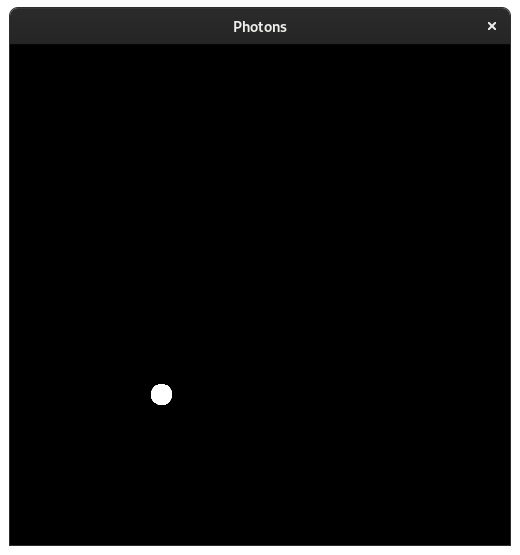
\includegraphics[width=\textwidth,trim={0 0 0 2cm},clip]{images/photons_1_01.png}
      \end{subfigure}
      \begin{subfigure}[b]{0.24\textwidth}
        \center
        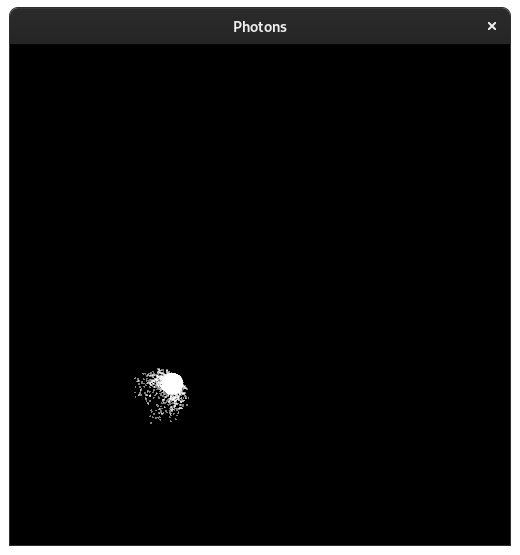
\includegraphics[width=\textwidth,trim={0 0 0 2cm},clip]{images/photons_1_02.png}
      \end{subfigure}
      \begin{subfigure}[b]{0.24\textwidth}
        \center
        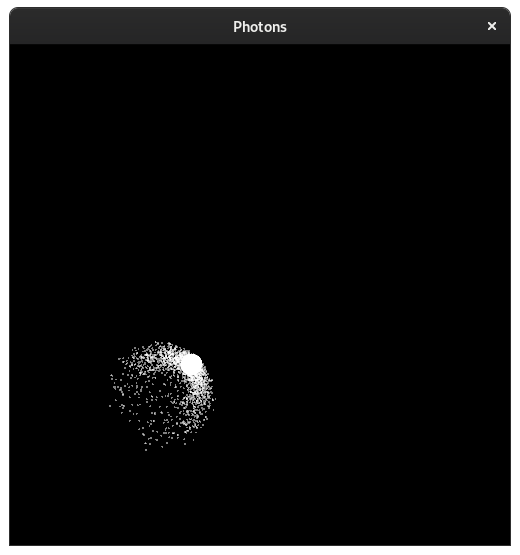
\includegraphics[width=\textwidth,trim={0 0 0 2cm},clip]{images/photons_1_03.png}
      \end{subfigure}
      \begin{subfigure}[b]{0.24\textwidth}
        \center
        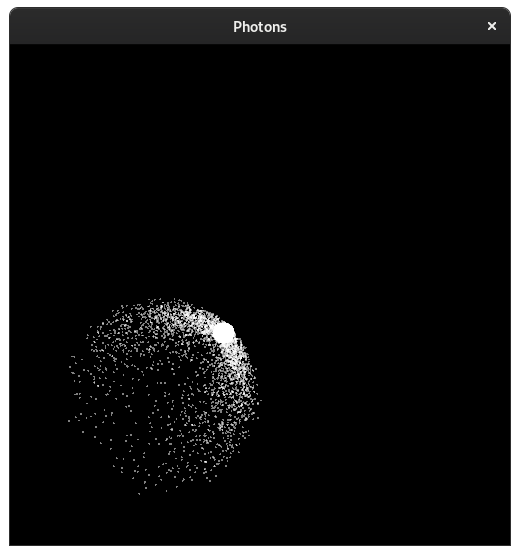
\includegraphics[width=\textwidth,trim={0 0 0 2cm},clip]{images/photons_1_04.png}
      \end{subfigure}
      \begin{subfigure}[b]{0.24\textwidth}
        \center
        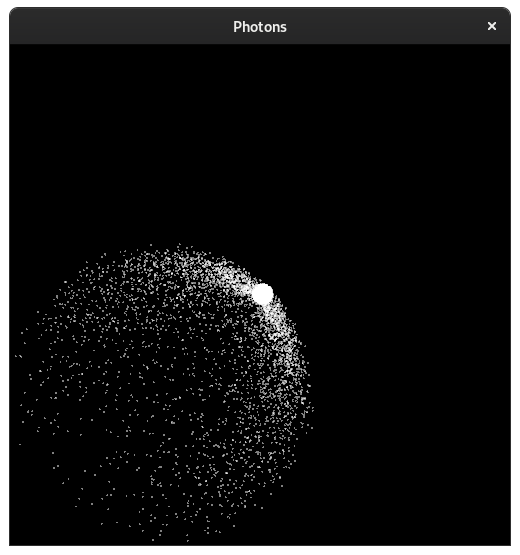
\includegraphics[width=\textwidth,trim={0 0 0 2cm},clip]{images/photons_1_05.png}
      \end{subfigure}
      \begin{subfigure}[b]{0.24\textwidth}
        \center
        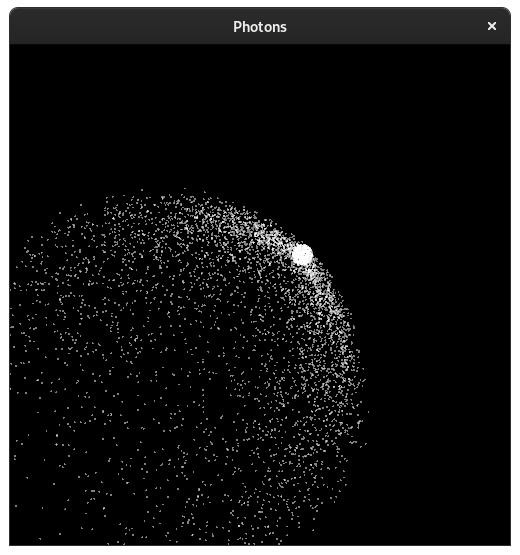
\includegraphics[width=\textwidth,trim={0 0 0 2cm},clip]{images/photons_1_06.png}
      \end{subfigure}
      \begin{subfigure}[b]{0.24\textwidth}
        \center
        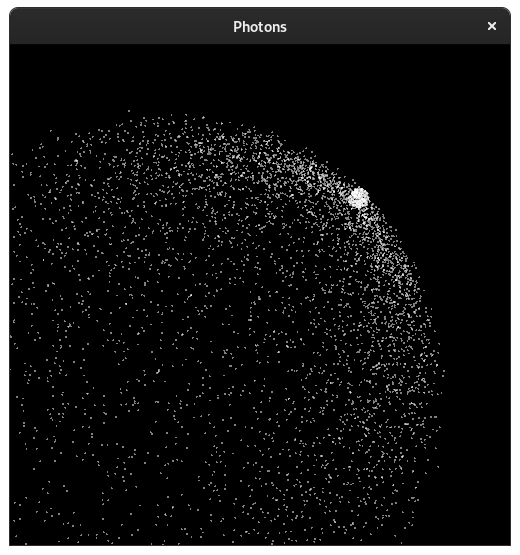
\includegraphics[width=\textwidth,trim={0 0 0 2cm},clip]{images/photons_1_07.png}
      \end{subfigure}
      \begin{subfigure}[b]{0.24\textwidth}
        \center
        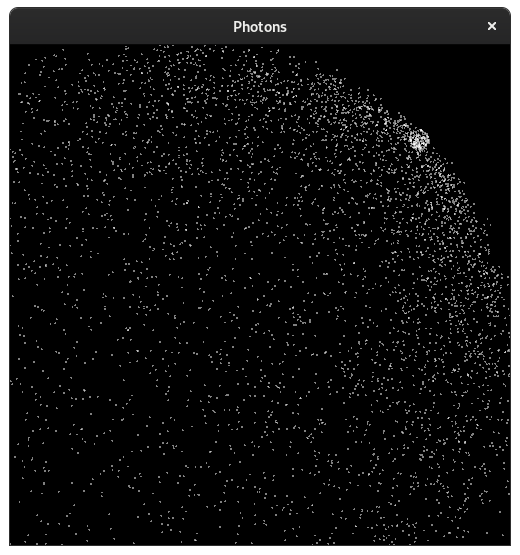
\includegraphics[width=\textwidth,trim={0 0 0 2cm},clip]{images/photons_1_08.png}
      \end{subfigure}
      \caption[Photon Simulation Time Evolution for Positive Asymmetry Parameter]{%
        Time evolution of the photon simulation for a positive asymmetry parameter.
        The initial state of the system is given by a ball of photons moving to the upper-right corner.
      }
      \label{fig:photons-time-evolution-positive}
    \end{figure}

    \begin{figure}[p]
      \center
      \begin{subfigure}[b]{0.24\textwidth}
        \center
        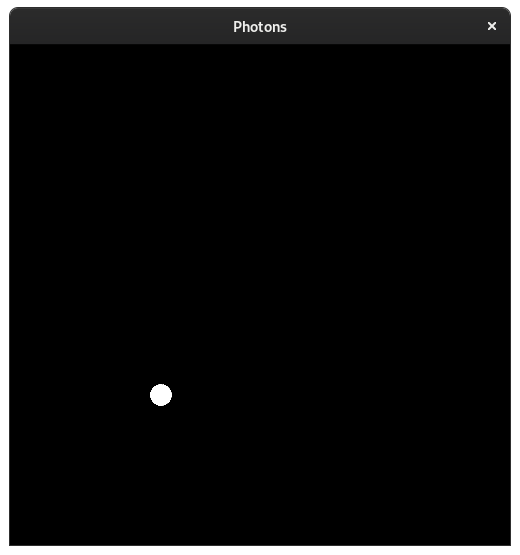
\includegraphics[width=\textwidth,trim={0 0 0 2cm},clip]{images/photons_2_01.png}
      \end{subfigure}
      \begin{subfigure}[b]{0.24\textwidth}
        \center
        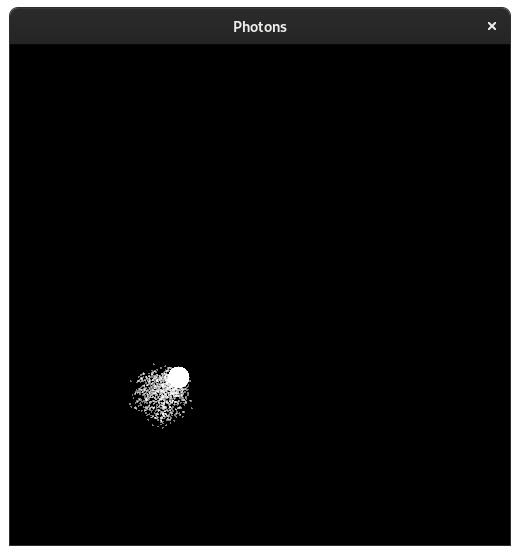
\includegraphics[width=\textwidth,trim={0 0 0 2cm},clip]{images/photons_2_02.png}
      \end{subfigure}
      \begin{subfigure}[b]{0.24\textwidth}
        \center
        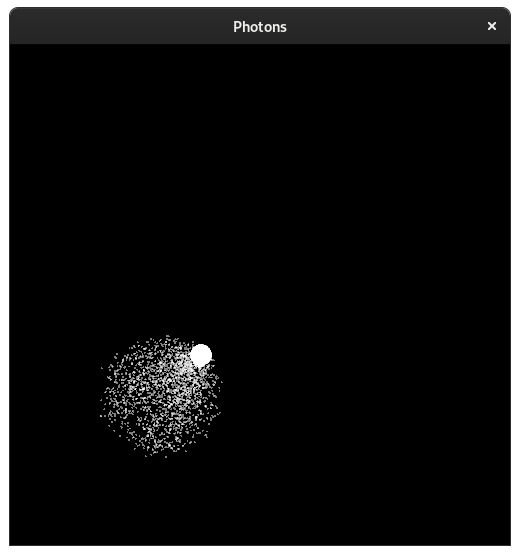
\includegraphics[width=\textwidth,trim={0 0 0 2cm},clip]{images/photons_2_03.png}
      \end{subfigure}
      \begin{subfigure}[b]{0.24\textwidth}
        \center
        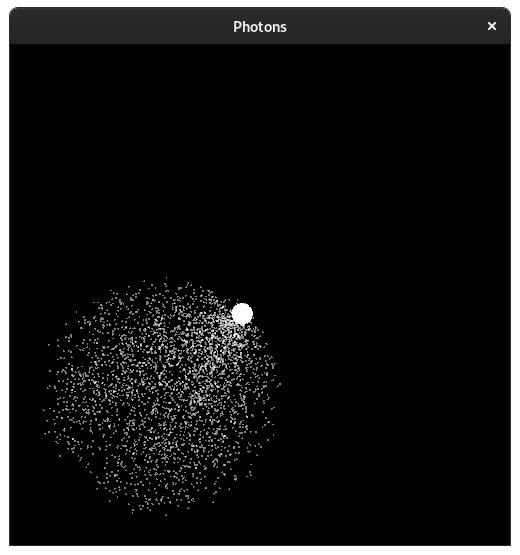
\includegraphics[width=\textwidth,trim={0 0 0 2cm},clip]{images/photons_2_04.png}
      \end{subfigure}
      \begin{subfigure}[b]{0.24\textwidth}
        \center
        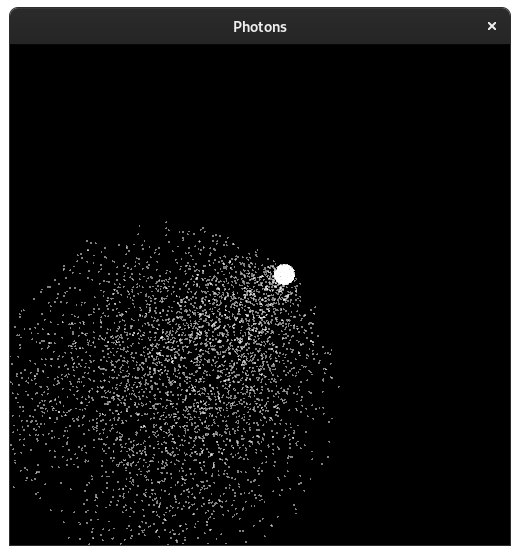
\includegraphics[width=\textwidth,trim={0 0 0 2cm},clip]{images/photons_2_05.png}
      \end{subfigure}
      \begin{subfigure}[b]{0.24\textwidth}
        \center
        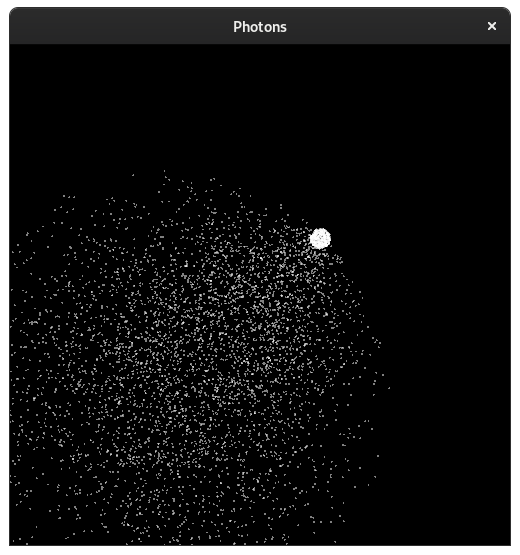
\includegraphics[width=\textwidth,trim={0 0 0 2cm},clip]{images/photons_2_06.png}
      \end{subfigure}
      \begin{subfigure}[b]{0.24\textwidth}
        \center
        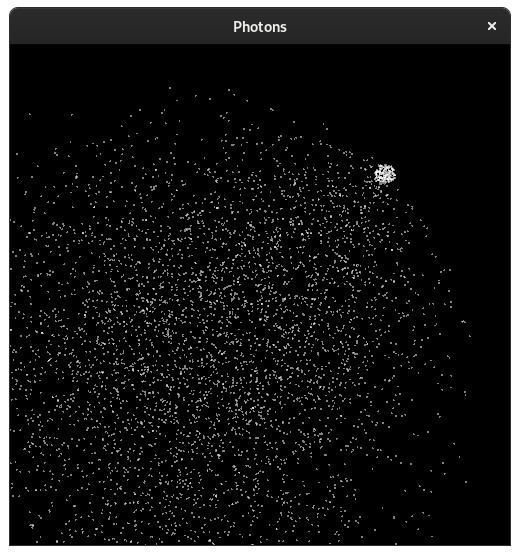
\includegraphics[width=\textwidth,trim={0 0 0 2cm},clip]{images/photons_2_07.png}
      \end{subfigure}
      \begin{subfigure}[b]{0.24\textwidth}
        \center
        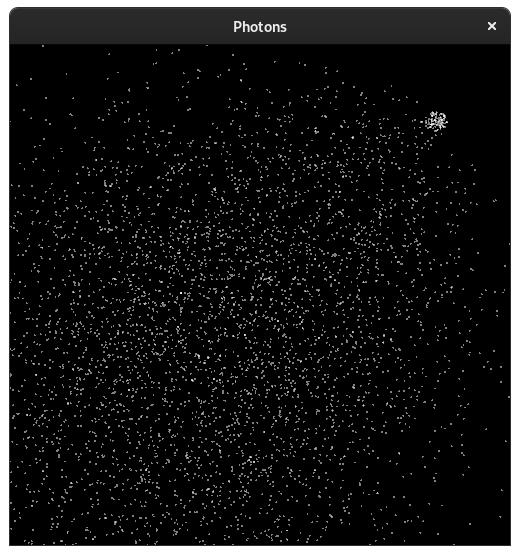
\includegraphics[width=\textwidth,trim={0 0 0 2cm},clip]{images/photons_2_08.png}
      \end{subfigure}
      \caption[Photon Simulation Time Evolution for Negative Asymmetry Parameter]{%
        Time evolution of the photon simulation for a negative asymmetry parameter.
        The initial state of the system is given by a ball of photons moving to the upper-right corner.
      }
      \label{fig:photons-time-evolution-negative}
    \end{figure}

    \inputCodeBlock[title = Photon Simulation Scalar Advancing]{code/photons/advance.hpp}
    The vectorization of this algorithm mostly consists of the interchanging of standard instructions with their according SIMD intrinsics.
    We have chosen to pack the positions and velocities of eight photons in AVX registers.
    Care has to be taken when translating the control branches.
    Using \code{_mm256_cmp_ps}, we can evaluate a condition for eight photons at the same time.
    The results are given as a mask.
    Thus, we execute the complete scattering transformation for all photons.
    At the end, we use \code{_mm256_blendv_ps} together with the mask to decide which part of the vector indeed has to be changed due to scattering.
    To show the need of vectorized PRNGs for applications that were already vectorized, we have created two different AVX versions.
    One version uses a scalar PRNG to generate its random numbers.
    The other version takes again a vectorized PRNG.
    Both variants are shown below.
    The complete implementation of the second version is given in the appendix in listing \ref{code:photons-avx-advance}.

    \inputCodeBlock[title = Scalar PRNG Call for AVX Implementation]{code/photons/scalar_call.hpp}

    \inputCodeBlock[title = AVX PRNG Call for AVX Implementation]{code/photons/avx_call.hpp}

  % subsection photon_benchmark (end)
% section testing_framework (end)
\end{document}